% 2008 年浙江卷文科第 20 题：矩形 ABCD 与梯形 BEFC 所在平面互相垂直，BE∥CF，
%   ∠BCF=∠CEF=90°，AD=√3，EF=2。
% 来源 PDF：gaokaomath-src/普通高考/2008/2008浙江文.pdf
% SHA-256：751204c132deb2b2f856ffeba082ce94063aa6e279783c2f07e4cd84539ecb63
% 原页：2008浙江文.pdf 第 2 页（A3 三栏）第 1 栏，书页码 494。
% 重绘依据：按斜投影作图，保持 AB∥DC、AD∥BC、BE∥CF；A 左上、B 左下、D 右上、C 居中、
%   E 在中下、F 在右下；可见棱 AB、AD、AC、AE、AF、DF、BE、EF 实线，自 C 出发的
%   BC、CD、CE、CF 被遮挡用虚线。
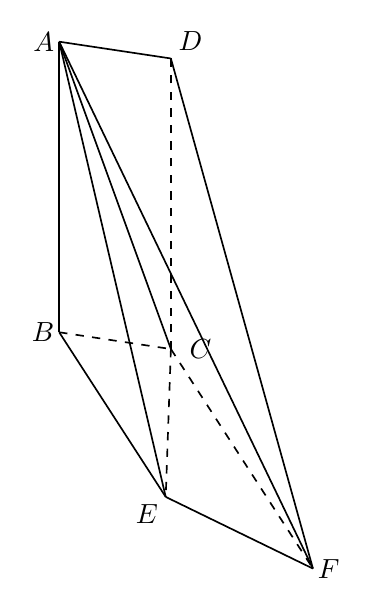
\begin{tikzpicture}[scale=0.82, semithick, every node/.style={inner sep=1.5pt}]
  \coordinate (A) at (1.00,8.50);
  \coordinate (B) at (1.00,4.00);
  \coordinate (C) at (2.73,3.74);
  \coordinate (D) at (2.73,8.24);
  \coordinate (E) at (2.65,1.45);
  \coordinate (F) at (4.93,0.34);

  % 可见棱
  \draw (A) -- (B);
  \draw (A) -- (D);
  \draw (A) -- (C);
  \draw (A) -- (E);
  \draw (A) -- (F);
  \draw (D) -- (F);
  \draw (B) -- (E);
  \draw (E) -- (F);

  % 被遮挡的棱（自 C 出发）
  \draw[dashed] (B) -- (C);
  \draw[dashed] (C) -- (D);
  \draw[dashed] (C) -- (E);
  \draw[dashed] (C) -- (F);

  \node[left] at (A) {$A$};
  \node[left] at (B) {$B$};
  \node[right=5pt] at (C) {$C$};
  \node[above right=1pt] at (D) {$D$};
  \node[below left=1pt] at (E) {$E$};
  \node[right] at (F) {$F$};
\end{tikzpicture}
